\documentclass[10pt, landscape]{article}
\usepackage[scaled=0.92]{helvet}
\usepackage{calc}
\usepackage{multicol}
\usepackage{ifthen}
\usepackage[a4paper,margin=3mm,landscape]{geometry}
\usepackage{amsmath,amsthm,amsfonts,amssymb}
\usepackage{color,graphicx,overpic}
\usepackage{hyperref}
\usepackage{newtxtext} 
\usepackage{enumitem}
\usepackage{amssymb}
\usepackage[table]{xcolor}
\usepackage{vwcol}
\usepackage{tikz}
\usetikzlibrary{arrows.meta}
\usetikzlibrary{calc}
\usepackage{mathtools}
\usepackage{nicematrix}
% for relations
\usepackage{cancel}
\usepackage{ mathrsfs }
\usepackage{minted}
\usemintedstyle{tango}
\definecolor{newblue}{HTML}{ADD8E6}
\colorlet{lightblue}{newblue!45}
\graphicspath{ {./images/} }
\setlist{nosep}

\pdfinfo{
  /Title (CS1101S.pdf)
  /Creator (TeX)
  /Producer (pdfTeX 1.40.0)
  /Author (Seamus)
  /Subject (Example)
  /Keywords (pdflatex, latex,pdftex,tex)}

% Turn off header and footer
\pagestyle{empty}

\newenvironment{tightcenter}{%
  \setlength\topsep{0pt}
  \setlength\parskip{0pt}
  \begin{center}
}{%
  \end{center}
}

% redefine section commands to use less space
\makeatletter
\renewcommand{\section}{\@startsection{section}{1}{0mm}%
                                {-1ex plus -.5ex minus -.2ex}%
                                {0.5ex plus .2ex}%x
                                {\normalfont\large\bfseries}}
\renewcommand{\subsection}{\@startsection{subsection}{2}{0mm}%
                                {-1explus -.5ex minus -.2ex}%
                                {0.5ex plus .2ex}%
                                {\normalfont\normalsize\bfseries}}
\renewcommand{\subsubsection}{\@startsection{subsubsection}{3}{0mm}%
                                {-1ex plus -.5ex minus -.2ex}%
                                {1ex plus .2ex}%
                                {\normalfont\small\bfseries}}%
\renewcommand{\familydefault}{\sfdefault}
\renewcommand\rmdefault{\sfdefault}
% makes nested numbering (e.g. 1.1.1, 1.1.2, etc)
\renewcommand{\labelenumii}{\theenumii}
\renewcommand{\theenumii}{\theenumi.\arabic{enumii}.}
\renewcommand\labelitemii{•}
%  for logical not operator
\renewcommand{\lnot}{\mathord{\sim}}
\renewcommand{\bf}[1]{\textbf{#1}}
\newcommand{\abs}[1]{\vert #1 \vert}
\newcommand{\Mod}[1]{\ \mathrm{mod}\ #1}

\makeatother
\definecolor{myblue}{cmyk}{1,.72,0,.38}
\everymath\expandafter{\the\everymath \color{myblue}}
% Define BibTeX command
\def\BibTeX{{\rm B\kern-.05em{\sc i\kern-.025em b}\kern-.08em
    T\kern-.1667em\lower.7ex\hbox{E}\kern-.125emX}}
\let\iff\leftrightarrow
\let\Iff\Leftrightarrow
\let\then\rightarrow
\let\Then\Rightarrow

% Don't print section numbers
\setcounter{secnumdepth}{0}

\setlength{\parindent}{0pt}
\setlength{\parskip}{0pt plus 0.5ex}
%% this changes all items (enumerate and itemize)
\setlength{\leftmargini}{0.5cm}
\setlength{\leftmarginii}{0.5cm}
\setlist[itemize,1]{leftmargin=2mm,labelindent=1mm,labelsep=1mm}
\setlist[itemize,2]{leftmargin=4mm,labelindent=1mm,labelsep=1mm}

%My Environments
\newtheorem{example}[section]{Example}
% -----------------------------------------------------------------------

\begin{document}
\raggedright
\footnotesize
\begin{multicols}{4}


% multicol parameters
% These lengths are set only within the two main columns
\setlength{\columnseprule}{0.25pt}
\setlength{\premulticols}{1pt}
\setlength{\postmulticols}{1pt}
\setlength{\multicolsep}{1pt}
\setlength{\columnsep}{2pt}

\begin{center}
    \fbox{%
        \parbox{0.8\linewidth}{\centering \textcolor{black}{
            {\Large\textbf{CS1101S}}
            \\ \normalsize{AY25/26 sem 1}}
            \\ {\footnotesize \textcolor{myblue}{github.com/lostmusician}} 
        }%
    }
\end{center}

\section{01 recursion}
\subsection{examples}
\begin{minted}[breaklines,breakanywhere,bgcolor=lightblue]{javascript}
function factorial(n) {
    if (n === 0) return 1; // base case
    return n * factorial(n - 1); // recursive case
}

function factorial(n) {
    return iter(1, 1, n);
}

function iter(product, counter, n) {
    return counter > n
        ? product // base case
        : iter(product * counter, counter + 1, n); // recursive case
}
\end{minted}
\begin{minted}[breaklines,breakanywhere,bgcolor=lightblue]{javascript}
function fib(n) {
    function f(n, k, x, y) {
        return (k > n)
            ? y
            : f(n, k + 1, y, x + y);
    }
    return (n < 2) ? n : f(n, 2, 0, 1);
}
\end{minted}

\begin{minted}[breaklines,breakanywhere,bgcolor=lightblue]{javascript}
function gcd(a, b) {
    return b === 0
        ? a
        : gcd(b, a % b);
}
\end{minted}
wishful thinking: assuming that the back is already solved

\subsection{CPS}
instead of letting the call stack remember, we explicitly pass a function c that encodes “what to do next.”
\begin{minted}[breaklines,breakanywhere,bgcolor=lightblue]{javascript}
function append_iter(xs, ys){
    // iterative process
    function app(xs, ys, c) {
        return is_null(xs)
        ? c(ys)
        : app(tail(xs), ys, 
              x => c(pair(head(xs), x))
              );
    }
    return app(xs, ys, x => x);
}
\end{minted}

\begin{minted}[breaklines,breakanywhere,bgcolor=lightblue]{javascript}
function fast_expt(b, n) {
    return n === 0
          ? 1
          : is_even(n)
          ? square(fast_expt(b, n / 2))
          : b * fast_expt(b, n - 1);
}

function fast_expt_cps(b, n, c) {
    return n === 0
          ? c(1)
          : is_even(n)
          ? fast_expt_cps(b, n / 2, x => c(square(x)))
          : fast_expt_cps(b, n - 1, x => c(b * x));
}
\end{minted}

\section{02 lists and trees}
A tree of certain data items is a list whose elements are such data items, or trees of such data items. \\
make tree takes 3 args: entry, left branch, right branch
\begin{minted}[breaklines,breakanywhere,bgcolor=lightblue]{javascript}
function BST_to_list(bst) {
    if (is_null(bst)) {
        return null;
    } else {
        const ltree = head(tail(bst));
        const num = head(bst);
        const rtree = head(tail(tail(bst)));
        return append(BST_to_list(ltree),
                      pair(num, BST_to_list(rtree)));
    }
}
\end{minted}

\begin{minted}[breaklines,breakanywhere,bgcolor=lightblue]{javascript}
function map_tree(f, tree) {
    return map(sub_tree => !is_list(sub_tree)
                ? f(sub_tree)
                : map_tree(f, sub_tree)
               , tree);
}
\end{minted}

\begin{minted}[breaklines,breakanywhere,bgcolor=lightblue]{javascript}
function flatten_tree(xs) {
    function h(xs, prev) {
        return is_null(xs)
            ? prev
            : is_list(xs)
                ? append(flatten_tree(xs), prev)
                : pair(xs, prev);
    }
    return accumulate(h, null, xs);
}
\end{minted}
\begin{minted}[breaklines,breakanywhere,bgcolor=lightblue]{javascript}
function insert(bst, item) {
    if (is_empty_tree(bst)) {
        return make_tree(item, 
                         make_empty_tree(), 
                         make_empty_tree());
    } else {
        if (item < entry(bst)) {
            // smaller than entry(left branch)
            return make_tree(entry(bst),
                       insert(left_branch(bst),
                              item),
                       right_branch(bst));
        } else if (item > entry(bst)) {
            // bigger than entry (right branch)
            return make_tree(entry(bst),
                       left_branch(bst),
                       insert(right_branch(bst),
                              item));
        } else {
            // equal to entry.
            return bst;
        }
    }
}
\end{minted}
\begin{minted}[breaklines,breakanywhere,bgcolor=lightblue]{javascript}
function find(bst, name) {
    return is_empty_tree(bst)
        ? false
        : name === entry(bst)
         ? true
         : name < entry(bst)
          ? find(left_branch(bst), name)
          : find(right_branch(bst), name);
}
\end{minted}

\subsection{matrix}
remember to use listref
\begin{minted}[breaklines,breakanywhere,bgcolor=lightblue]{javascript}
function transpose(M) {
    const nR = length(M); // number of rows
    const nC = length(head(M)); // columns
    return map(c => map(row => list_ref(row, c), M), enum_list(0, nC - 1));
}

function row_sums(M) {
    return map(row => accumulate((x, sum) => x + sum, 0, row), M);
}
\end{minted}

\begin{minted}[breaklines,breakanywhere,bgcolor=lightblue]{javascript}
function map_using_accumulate(f, xs) {
    return accumulate((x, result) => 
                pair(f(x), result), null, xs);
}

function filter_using_accumulate(pred, xs) {
    return accumulate(
        (x, result) => pred(x) 
        ? pair(x, result) : result,
        null,
        xs
    );
}
\end{minted}

\section{03 permutations and combinations}
\begin{minted}[breaklines,breakanywhere,bgcolor=lightblue]{javascript}
function permutations(s) {
    return is_null(s)
        ? list(null)
        : accumulate(append, null,
                     map(x => map(p => pair(x, p),
                     permutations(remove(x, s))),
                     s));
}


function subsets(s) {
    return accumulate(
        (x, s1) => append(s1,
                   map(ss => pair(x, ss), s1)),
        list(null),
        s);
}
function choose(n, r) {
    if (n < 0 || r < 0) {
        return 0;
    } else if (r === 0) {
        return 1;
    } else {
        // Consider the 1st item, there are 2 choices:
        // To use, or not to use
        // Get remaining items with wishful thinking
        const to_use = choose(n - 1, r - 1);
        const not_to_use = choose(n - 1, r);
        
        return to_use + not_to_use;
    }
}

function combinations(xs, r) {
    if ( (r !== 0 && xs === null) || r < 0) {
        return null;
    } else if (r === 0) {
        return list(null);
    } else {
        const no_choose = combinations(tail(xs), r);
        const yes_choose = combinations(tail(xs),
                                        r - 1);
        const yes_item = map(x => pair(head(xs), x),
                             yes_choose);
        return append(no_choose, yes_item);
    }
}
\end{minted}

\section{04 sorting algorithms}
insertion, selection, quicksort, mergesort
\begin{minted}[breaklines,breakanywhere,bgcolor=lightblue]{javascript}
function insert(x, xs) {
    return is_null(xs)
        ? list(x)
        : x <= head(xs)
            ? pair(x, xs)
            : pair(head(xs), insert(x, tail(xs)));
}

function insertion_sort(xs) {
    return is_null(xs)
        ? xs
        : insert(head(xs),
                 insertion_sort(tail(xs)));
}
\end{minted}
Insertion sort: Builds the sorted list one item at a time by taking each element and inserting it into its correct place among the already-sorted elements.

\begin{minted}[breaklines,breakanywhere,bgcolor=lightblue]{javascript}
function selection_sort(xs) {
    if (is_null(xs)) {
        return xs;
    } else {
        const x = smallest(xs);
        return pair(x,
            selection_sort(remove(x, xs)));
    }
}

function smallest(xs) {
    function h(xs, min) {
        return xs === null
            ? min
            : head(xs) < min
                ? h(tail(xs), head(xs))
                : h(tail(xs), min);
    }
    return h(xs, head(xs));
}
\end{minted}
Selection sort: Repeatedly finds the minimum (or maximum) element from the unsorted part and puts it at the beginning.

\begin{minted}[breaklines,breakanywhere,bgcolor=lightblue]{javascript}
function partition(xs, p) {
    function h(xs, lte, gt) {
        if (is_null(xs)) {
            return pair(lte, gt);
        } else {
            const first = head(xs);
            return first <= p
                ? h(tail(xs), pair(first, lte), gt)
                : h(tail(xs), lte, pair(first, gt));
        }
    }
    return h(xs, null, null);
}


function quicksort(xs) {
    if (is_null(xs) || is_null(tail(xs))) {
        return xs;
    } else {
        const pivot = head(xs);
        const splits = partition(tail(xs), pivot);
        const smaller = quicksort(head(splits));
        const bigger = quicksort(tail(splits));
        return append(smaller, pair(pivot, bigger));
    }
}
\end{minted}
Quick sort: Picks a pivot element, partitions the list into elements less than the pivot and greater than the pivot, then recursively sorts the partitions.

\begin{minted}[breaklines,breakanywhere,bgcolor=lightblue]{javascript}
function take(xs, n) {
    return n === 0
        ? null
        : pair(head(xs),
               take(tail(xs), n - 1));
}
function drop(xs, n) {
    return n === 0
        ? xs
        : drop(tail(xs), n - 1);
}

function merge(xs, ys) {
    if (is_null(xs)) { 
        return ys;
    } else if (is_null(ys)) { 
        return xs;
    } else {
        const x = head(xs);
        const y = head(ys);
        return (x < y) 
            ? pair(x, merge(tail(xs), ys))
            : pair(y, merge(xs, tail(ys)));
    }
}

function merge_sort(xs) {
    if (is_null(xs) || is_null(tail(xs))) {
        return xs;
    } else {
        const mid = math_floor(length(xs) / 2);  
        return merge(merge_sort(take(xs, mid)), 
                     merge_sort(drop(xs, mid)));
    }
}
\end{minted}
Merge sort: Recursively splits the list in half, sorts each half, then merges the two sorted halves back together.

\section{05 time complexity identifiers} 
\begin{center}
    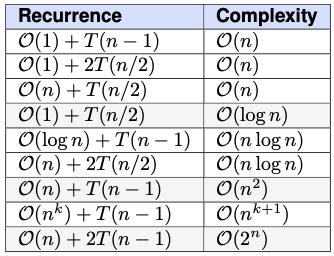
\includegraphics[width=\linewidth]{recurrence relation.png}
\end{center}

\begin{center}
    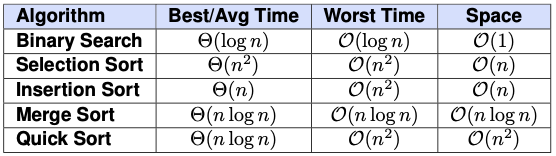
\includegraphics[width=\linewidth]{sorts time complexities.png}
Time complexity will always be greater than or equal to space complexity since we need time to create space.
\end{center}


\begin{center}
    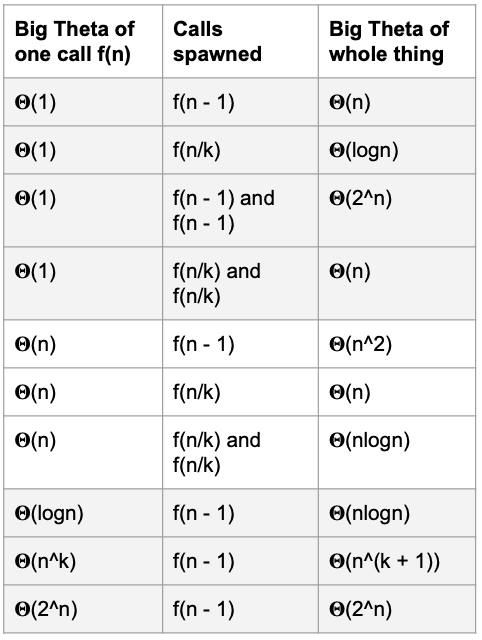
\includegraphics[width=\linewidth]{TA hax.png}
\end{center}

\section{06 T diagrams} 
 \begin{center}
    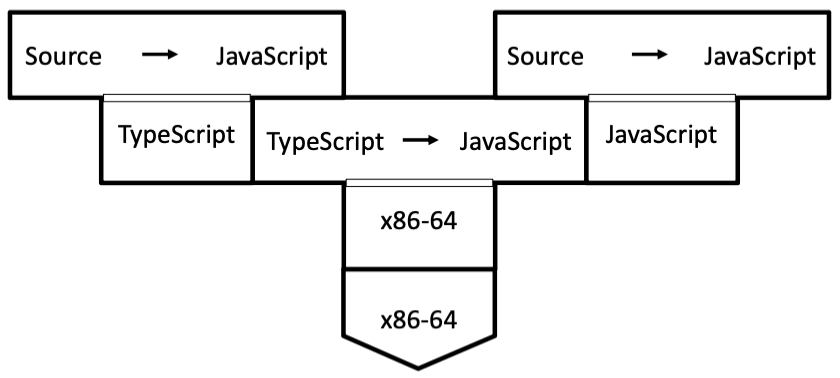
\includegraphics[width=\linewidth]{compiling compiler.png}
compiling a compiler
\end{center}

\begin{center}
    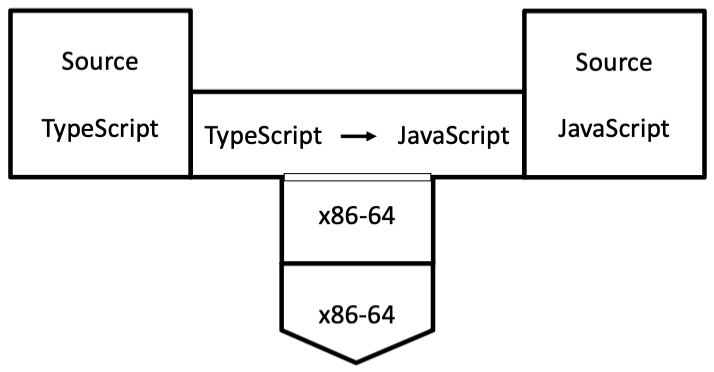
\includegraphics[width=\linewidth]{compiling stepper.png}
compiling the stepper from TS to JS
\end{center}


\begin{center}
    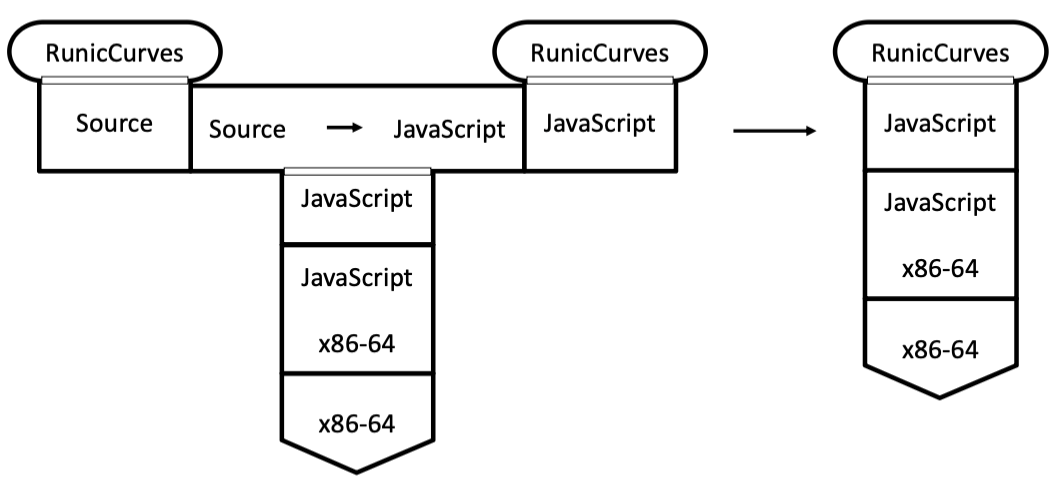
\includegraphics[width=\linewidth]{compiling and executing web program.png}
compiling and executing a web program
\end{center}

\begin{center}
    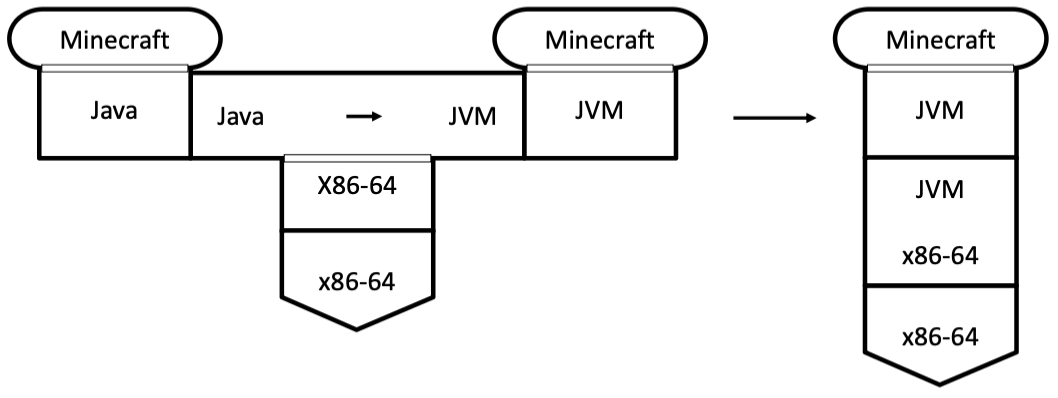
\includegraphics[width=\linewidth]{compiling and executing program.png}
compiling and executing a program
\end{center}

\end{multicols}

\end{document}